\begin{wrapfigure}[0]{r}[-1cm]{3cm}
 \vspace{-6cm}
 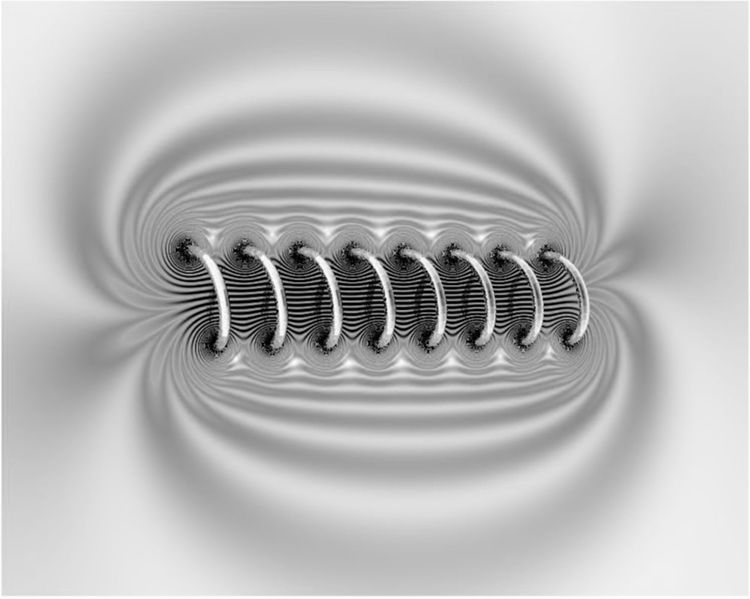
\includegraphics[scale=0.25]{elektromagnetisch/Bilder/750px-Solenoid-6.jpg}
 \vspace{-6cm}
\end{wrapfigure}

\section*{Theorie- und Prüfungsfragen} 

\mucho{1}{TB305}
{Wie nennt man das Feld zwischen zwei parallelen Kondensatorplatten bei Anschluss einer Gleichspannung?}%Frage
{Homogenes elektrisches Feld}%A
{Homogenes magnetisches Feld}%B
{Polarisiertes elektrisches Feld}%C
{Polarisiertes magnetisches Feld}%D
{A}%Lösung

\mucho{2}{TB406}
{Wenn Strom durch einen gestreckten Leiter fließt, entsteht ein}%Frage
{homogenes Magnetfeld um den Leiter.}%A
{elektrisches Feld aus konzentrischen Kreisen um den Leiter.}%B
{Magnetfeld aus konzentrischen Kreisen um den Leiter.}%C
{homogenes elektrisches Feld um den Leiter.}%D
{C}%Lösung

\mucho{3}{TB405}
{Wie nennt man das Feld im Innern einer langen Zylinderspule beim Fließen eines Gleichstroms?}
{Homogenes magnetisches Feld}%A
{Homogenes elektrisches Feld}%B
{Konzentrisches magnetisches Feld}%C
{Zentriertes magnetisches Feld}%D
{A}%Lösung


\mucho{4}{TB502}
{Wie erfolgt die Ausbreitung einer elektromagnetischen Welle? (Im folgenden Text ist H-Feld die magnetische Feldkomponente und E-Feld die elektrische Feldkomponente.)}%Frage
{Sie erfolgt durch eine sich ausbreitende Wechselwirkung zwischen E-Feld und H-Feld.}%A
{Die Ausbreitung erfolgt nur über das E-Feld. Das H-Feld ist nur im Nahfeld vorhanden.}%B
{Die Ausbreitung erfolgt nur über das H-Feld. Das E-Feld ist nur im Nahfeld vorhanden.}%C
{E-Feld und H-Feld breiten sich unabhängig voneinander aus und stehen senkrecht zueinander und zur Ausbreitungsrichtung.}%D
{A}%Lösung


\mucho{5}{TB511}
{Eine Yagiantenne mit 12,15 dBi Antennen- gewinn wird mit 250 W Senderleistung direkt gespeist. Welche elektrische Ersatzfeldstärke ergibt sich bei Freiraumausbreitung in 30 m Entfernung?}%Frage
{9,2 V/m}%A
{11,8 V/m}%B
{13,1 V/m}%C
{353 V/m}%D
{B; $P_{EIRP} = P_S \cdot 10^{\frac{g_i}{10}}; E=\dfrac{\sqrt{30\Omega \cdot P_{EIRP}}}{d}$}%Lösung

\mucho{6}{TI101}
{Welche ionosphärischen Schichten bestimmen die Fernausbreitung am Tage?}%Frage
{D-, E-, F1- und F2-Schicht}%A
{E- und F-Schicht}%B
{F1- und F2-Schicht}%C
{E- und D-Schicht}%D
{A}%Lösung

\mucho{7}{TI237}
{ Warum sind Signale im 160-, 80- und 40-Meter-Band tagsüber nur schwach und nicht für den weltweiten Funkverkehr geeignet?}%Frage
{Wegen der Tagesdämpfung in der D-Schicht.}%A
{Wegen der Tagesdämpfung in der F1-Schicht.}%B
{Wegen der Tagesdämpfung in der F2-Schicht.}%C
{Wegen der Tagesdämpfung in der A-Schicht.}%D
{A}%Lösung

\mucho{8}{TI237}
{Was bedeutet der Begriff ``Sporadic E''? Es ist}%Frage
{eine Reflexion an lokal begrenzten Bereichen mit ungewöhnlich hoher Ionisation innerhalb der E-Schicht.}%A
{eine kurzfristige, plötzliche Inversionsänderung in der E-Schicht, die Fernausbreitung im VHF-Bereich ermöglicht.}%B
{eine kurzzeitig auftretende, starke Reflexion von VHF-Signalen an Meteorbahnen innerhalb der E-Schicht.}%C
{ein lokal begrenzter, kurzzeitiger Ausfall der Reflexion durch ungewöhnlich hohe Ionisation innerhalb der E-Schicht.}%D
{A}%Lösung

\mucho{9}{TI224}
{Die MUF für eine Funkstrecke ist}%Frage
{der Mittelwert aus der höchsten und niedrigsten brauchbaren Frequenz, bei der sich elektro­magnetische Wellen zwischen zwei Orten durch ionosphärische Brechung ausbreiten können.}%A
{die niedrigste brauchbaren Frequenz, bei der sich elektromagnetische Wellen zwischen zwei Orten durch ionosphärische Brechung ausbreiten können.}%B
{die vorgeschriebene nutzbare Frequenz bei der sich elektromagnetische Wellen zwischen zwei Orten durch ionosphärische Brechung ausbreiten können.}%C
{die höchste brauchbare Frequenz, bei der sich elektromagnetische Wellen zwischen zwei Orten durch ionosphärische Brechung ausbreiten können.}%D
{D}%Lösung

\mucho{10}{TI213}
{Was versteht man unter dem Begriff ``Mögel-Dellinger-Effekt''? Man versteht darunter}%Frage
{das Übersprechen der Modulation eines starken Senders auf andere, über die Ionosphäre übertragene HF-Signale.}%A
{den zeitlich begrenzten Schwund durch Mehrwegeausbreitung in der Ionosphäre.}%B
{die zeitlich begrenzt auftretende Verzerrung der Modulation.}%C
{den totalen, zeitlich begrenzten Ausfall der Reflexion an der Ionosphäre.}%D
{D}%Lösung
